\section{Elektromagnetiska vågor}
Från Maxwells ekvationer kan man visa att flera storheter kopplade till elektromagnetism följer vågekvationen. Dessa vågor kallas för elektromagnetiska vågor. Experimenter visade att ljus propagerade med samma farten som den teoretiska farten till elektromagnetiska vågor, och därmed blev det snabbt etablerat att ljus är elektromagnetiska vågor. Därmed kommer vi ägna en hel sektion åt att diskutera de.

\subsection{Principer}

\paragraph{Essensiell information från Maxwells ekvationer}
Från Maxwells ekvation får man veta att
\begin{itemize}
	\item elektromagnetiska vågor är transversella.
	\item elektromagnetiska vågor utbredar sig med ljusfarten $c = \frac{1}{\sqrt{\varepsilon_0\mu_0}}$ i vakuum, och motsvarande i andra media.
	\item $\vect{B}\perp\vect{E}$.
	\item $B = \frac{1}{c}E$.
	\item $\vect{E}\times\vect{B}$ pekar i utbridningsriktningen.
\end{itemize}

\paragraph{Fermats princip}
Strålgången till ljus mellan två punkter följer den snabbaste vägen.

\paragraph{Dispersion}
Dispersion är när ett mediums brytningsindex beror på vågens våglängd.

\paragraph{Polarisation}
Elektriskt och magnetiskt fält är vektorstorheter, och det betyder att de kan svänga i olika plan. Ljusets polarisation refererar till hur fälterna svängar i planet normalt på utbridgningen.

Ljus kan vara
\begin{itemize}
	\item linjärpolariserat, så att fältet oscillerar på en linje i det normala planet.
	\item elliptiskt polariserat, så att fältet oscillerar på en ellips i det normala planet.
	\item opolariserat, så att fältet oscillerar godtyckligt utan preferens för någon riktning.
\end{itemize}

\paragraph{Dubbeltbrytande material}
Ett dubbeltbrytande material har brytningsindex som beror på polarisationen.

\paragraph{Optisk aktivitet}
Det finns väl typ saker som kan vrida polarisationsriktningen på polariserat ljus, eller någonting.

\subsection{Ekvationer}

\paragraph{Vågekvationen för $\vect{E}$}
\begin{align*}
	\laplacian{\vect{E}} = \varepsilon\mu\pdv{\vect{E}}{t}
\end{align*}

\deriv

\paragraph{Definitionen av brytningsindex}
\begin{align*}
	n = \frac{c_0}{c}
\end{align*}
Här är $c_0$ ljusfarten i vakuum. Per definition är $n\geq 1$ i linjära materialer. Definitionen ger
\begin{align*}
	n = \sqrt{\varepsilon_{\text{r}}\mu_{\text{r}}}
\end{align*}
där $\varepsilon_{\text{r}}, \mu_{\text{r}}$ är relativa permeabiliteter och permittiviteter.

\paragraph{Reflektionskoefficient för elektromagnetiska vågor}
\begin{align*}
	R = \left(\frac{n_1 - n_2}{n_1 + n_2}\right)^2
\end{align*}

\paragraph{Våglängd i medium}
\begin{align*}
	\lambda = \frac{\lambda_0}{n}
\end{align*}
$\lambda_0$ är våglängden i vakuum. En direkt konsekvens av detta är att
\begin{align*}
	k = nk_0
\end{align*}
för vågvektorn, där $k_0$ är vågvektorns längd i vakuum.

\deriv
Vi har från innan att vid transmission mellan två medier ändras inte frekvens. Detta ger att
\begin{align*}
	\lambda = \frac{c}{f} = \frac{c_0}{nf} = \frac{\lambda_0}{n}
\end{align*}
där $c_0$ är vågfarten i vakuum.

\paragraph{Definitionen av optisk väg}
För en given bana definieras den optiska vägen ljus tar som
\begin{align*}
	L = \int\limits_{C}\dd{l}n,
\end{align*}
som för materialer med konstant brytningsindex reduceras till
\begin{align*}
	L = \sum L_in_i,
\end{align*}
där $L_i$ är sträckan vägen rör sig i materialet med brytningsindex $n_i$.

\paragraph{Poyntingvektorn}
\begin{align*}
	\vect{S} = \frac{1}{\mu_0}\vect{E}\times\vect{B}
\end{align*}
Poyntingvektorn ger information om energitransport från en elektromagnetisk våg. Dens riktning indikerar i vilken riktning energin transporteras, och dens belopp indikerar hur mycket energi som transporteras. I den kompleksa formalismen definieras den som
\begin{align*}
	\vect{S} = \frac{1}{2\mu_0}\vect{E}*\times\vect{B}.
\end{align*}

\deriv
I ett litet tidsintervall flödar energin
\begin{align*}
	\dd{U} = u\dd{V} = uAc\dd{t}
\end{align*}
genom arean $A$. För en elektromagnetisk våg har man
\begin{align*}
	u = \frac{1}{2}\varepsilon_0E^2 + \frac{1}{2\mu_0}B^2.
\end{align*}
Med relationen $B = \frac{E}{c}$ får man
\begin{align*}
	u = \varepsilon_0E^2,
\end{align*}
vilket ger
\begin{align*}
	\dd{U} = u\dd{V} = \varepsilon_0E^2Ac\dd{t}.
\end{align*}
Flödet per tidsenhet och area ges av
\begin{align*}
	S = \frac{1}{A}\dv{U}{t} = \frac{EB}{\mu_0}.
\end{align*}
Givet detta, definierar man
\begin{align*}
	\vect{S} = \frac{1}{\mu_0}\vect{E}\times\vect{B}
\end{align*}
som uppfyller
\begin{align*}
	\abs{\vect{S}} = \frac{EB}{\mu_0}
\end{align*}
och vars riktning även ger information om i vilken riktning energin transporteras. Denna vektorn används som inspiration till definitionen i den komplexa beskrivningen.

\paragraph{Intensitet för elektromagnetisk våg}
\begin{align*}
	I = \frac{1}{2}\varepsilon_0cE^2
\end{align*}

\deriv
Enligt definitionen är
\begin{align*}
	I = \expval{S}.
\end{align*}
För enkla harmoniska fält har man
\begin{align*}
	\abs{\vect{S}} = \frac{1}{2\mu_0}\vect{E}*\times\vect{B} = \frac{E^2}{2c\mu_0}.
\end{align*}
Detta ger
\begin{align*}
	I = \expval{S} = \frac{E^2}{2c\mu_0}.
\end{align*}

\paragraph{Malus' lag}
Om ljus med intensitet $I_0$ skickas in på en polariserande skärm, har ljuset på andra sidan intensitet
\begin{align*}
	I = I_0\cos^2{\theta}.
\end{align*}
$\theta$ är vinkeln det inkommande ljusets polarisation bildar med skärmens polarisationsriktning.

\deriv
Följer av att $I\propto E^2$ och att en polariserande skärm fjärnar komponenten av $\vb{E}$ som är normal på skärmens polarisationsriktning.

\paragraph{Fresnels formler}
\begin{align*}
	\frac{E_{\text{rp}}}{E_{\text{ip}}} &= \frac{\tan{(\theta_{\text{i}} - \theta_{\text{b}})}}{\tan{(\theta_{\text{i}} + \theta_{\text{b}})}} \\
	\frac{E_{\text{tp}}}{E_{\text{ip}}} &= \frac{2\sin{(\theta_{\text{b}})}\cos{(\theta_{\text{i}})}}{\sin{(\theta_{\text{i}} + \theta_{\text{b}})}\cos{(\theta_{\text{i}} - \theta_{\text{b}})}} \\
	\frac{E_{\text{rs}}}{E_{\text{is}}} &= -\frac{\sin{(\theta_{\text{i}} - \theta_{\text{b}})}}{\sin{(\theta_{\text{i}} + \theta_{\text{b}})}} \\
	\frac{E_{\text{ts}}}{E_{\text{is}}} &= \frac{2\sin{(\theta_{\text{b}})}\cos{\theta_{\text{i}})}}{\sin{(\theta_{\text{i}} + \theta_{\text{p}})}}
\end{align*}
Det första indexet indikerar om ljuset är reflekterat eller transmitterat. Det andra indexet indikerar om ljuset är polariserat parallellt eller normalt mot infallsplanet.

\deriv
Fås från gränsvillkoren för elektriskt och magnetiskt fält.

\paragraph{Brewstervinkeln}
När ljus skickas in på en gränsyta med infallsvinkeln $\theta_{\text{B}}$ så att
\begin{align*}
	\tan{\theta_{\text{B}}} = \frac{n_2}{n_1}
\end{align*}
är det reflekterade ljuset linjärpolariserat vinkelrät mot infallsplanet. Denna vinkeln kallas Brewstervinkeln.

\deriv
Fresnels formler ger att $E_{\text{rp}} = 0$ när $\theta_{\text{i}} + \theta_{\text{b}} = \frac{\pi}{2}$. Brytningslagen ger då
\begin{align*}
	\frac{\sin{\theta_{\text{i}}}}{\sin{\theta_{\text{b}}}} = \frac{\sin{\theta_{\text{i}}}}{\sin{\left(\frac{\pi}{2} - \theta_{\text{i}}\right)}} = \frac{\sin{\theta_{\text{i}}}}{\cos{\theta_{\text{i}}}} = \frac{c_{1}}{c_{2}}.
\end{align*}
Från definitionen av brytningsindex får man då
\begin{align*}
	\tan{\theta_{\text{i}}} = \frac{n_2}{n_1}.
\end{align*}
Vinkeln som uppfyller detta döps till $\theta_{\text{B}}$.

\paragraph{Tunnfilminterferens}
Betrakta figur \ref{fig:thin-film}.
\begin{figure}[!ht]
	\centering
	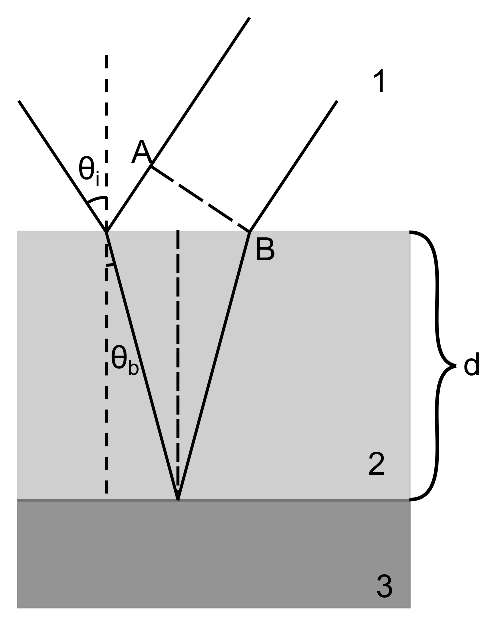
\includegraphics[scale=1]{./Images/thin-film/thin-film.eps}
	\caption{Illustration av strålbanan vid tunnfilmsinterferens.}
	\label{fig:thin-film}
\end{figure}

Om man antar att det ej händer reflektion i medium 3, är den optiska vägskillnaden mellan de två ritade punkterna
\begin{align*}
	\Delta L &= 2n_2\frac{d}{\cos{\theta_{\text{b}}}} - 2n_1d\tan{\theta_{\text{b}}}\sin{\theta_{\text{i}}} \\
	         &= 2n_2\frac{d}{\cos{\theta_{\text{b}}}} - 2n_2\sin{\theta_{\text{b}}}d\tan{\theta_{\text{b}}} \\
	         &= 2n_2\frac{d}{\cos{\theta_{\text{b}}}}\left(1 -\sin^2{\theta_{\text{b}}}\right) \\
	         &= 2n_2d\cos{\theta_{\text{b}}}.
\end{align*}

För att beräkna det äntliga interferensmönsteret, måste man även betrakta fassprang i gränsytorna.